\documentclass[UTF8,AutoFakeBold,a4paper]{article}
\usepackage{ctex}
\usepackage{framed}
\usepackage{amsthm}
\usepackage{geometry}
\usepackage{amsthm,amsmath,amssymb}
\usepackage{mathrsfs}
\geometry{left=2.5cm,right=2.5cm,top=2.5cm,bottom=2.5cm}
\usepackage{amsmath}
\usepackage{graphicx}
\usepackage{subfiles}
\linespread{1.314}
%\usepackage{luatexja-fontspec}
\setCJKmainfont[ItalicFont=FandolKai-Regular,BoldFont=STSongti-SC-Black]{SimSun} 
\usepackage{physics}
\usepackage{graphicx}
\setCJKfamilyfont{kaiti}{FandolKai-Regular}
\newcommand{\kaiti}{\CJKfamily{kaiti}}%
\usepackage{paralist}
\everymath{\displaystyle}
\usepackage{chngcntr}%图片编号的宏包
\counterwithout{figure}{section}%取消图片按章节编号
\counterwithin{figure}{section}%将equation环境重新编号,不按节编号
%\usepackage{emoji}
%\usepackage{ntheorem}
%\setemojifont{Twemoji Mozilla} 
%
%\usepackage{multicol}
%\let\itemize\compactitem
%\let\enditemize\endcompactitem
%\let\enumerate\compactenum
%\let\endenumerate\endcompactenum
%\let\description\compactdesc
%\let\enddescription\endcompactdesc
\usepackage{color}
\usepackage{fancyhdr} %调用宏包

% ---基本设置---

%设定页面的页眉页脚类型,$\LaTeX$内置了四种:empty、plain、headings及myheadings
\pagestyle{fancy}

%清除原页眉页脚样式
\fancyhf{} 

%R:页面右边;O:奇数页;\leftmark:表示“一级标题”
\fancyhead[CO]{\leftmark}

%L:页面左边;E:偶数页;\rightmark:表示“二级标题”
\fancyhead[CE]{\rightmark}

%C:页面中间
\fancyhead[CO, CE]{物理化学实验数据处理}

% 设置页脚,页眉的位置上也可以放置页码
\fancyfoot[CO]{\thepage}

% 设置页眉页脚横线及样式
%页眉线宽,设为0可以去页眉线
\renewcommand{\headrulewidth}{0.5pt} 

\usepackage{listings}

{
\lstset{numbers=left, %设置行号位置
        numberstyle=\zihao{-5}, %设置行号大小
        keywordstyle=\textcolor[rgb]{0.07,0.36,0.57}, %设置关键字颜色
        commentstyle=\textcolor[rgb]{0.21,0.49,0.30}, %设置注释颜色
        escapeinside=``, %逃逸字符(1左面的键),用于显示中文
        extendedchars=false, 
        xleftmargin=2em,xrightmargin=2em, aboveskip=1em, %设置边距
        tabsize=4, %设置tab空格数
        showspaces=false %不显示空格
       }

\title{\textbf{物理化学实验}}
\date{\today}
\author{B.H.Zhang}
%\setmainfont{Times New Roman}
%\setCJKsansfont{STSong}
%%\setCJKmainfont[BoldFont=STHeiti]{STSong}
%%\setCJKmainfont{STXihei}
%\setCJKmonofont{STXihei}
\usepackage{chemfig}
\usepackage{mathrsfs}
\usepackage{listings}
\usepackage{makeidx}
\makeindex
\usepackage{framed}
\usepackage{amsthm,amsmath,amssymb}
\usepackage{wrapfig}
\usepackage{graphicx}
\usepackage{mathrsfs}
\bibliographystyle{plain}
\usepackage{subfiles}
\usepackage{booktabs}
\usepackage{graphicx,times}
\usepackage{esint}
\usepackage{times}
\usepackage{subfigure}         
\usepackage{natbib}
\usepackage{amssymb,amsmath}
\usepackage{url}
\usepackage{geometry}
\usepackage{xcolor}
\usepackage{setspace}
\usepackage{subfigure}
\usepackage{booktabs}
\usepackage{array}
\usepackage{mhchem}
%\usepackage[usenames,dvipsnames]{color}
\usepackage{colortbl}
\usepackage{bm}
\usepackage{calligra}
\definecolor{mygray}{gray}{.9}
\definecolor{mypink}{rgb}{.99,.91,.95}
\definecolor{mycyan}{cmyk}{.3,0,0,0}
\definecolor{myorgn}{rgb}{0.56,0.28,0.16}
\definecolor{myyelo}{rgb}{255,215,0}
\usepackage{environ}
\everymath{\displaystyle}  
\usepackage[breaklinks,colorlinks,linkcolor=black,citecolor=black,urlcolor=black]{hyperref}
\usepackage{tikz}
\begin{document}
	\maketitle
	\section{}
	\section{}
	\section{}
	\section{}
	\section{}
	
	\section{实验六:原电池电动势的测定}
	\begin{figure}[h]
	\centering
	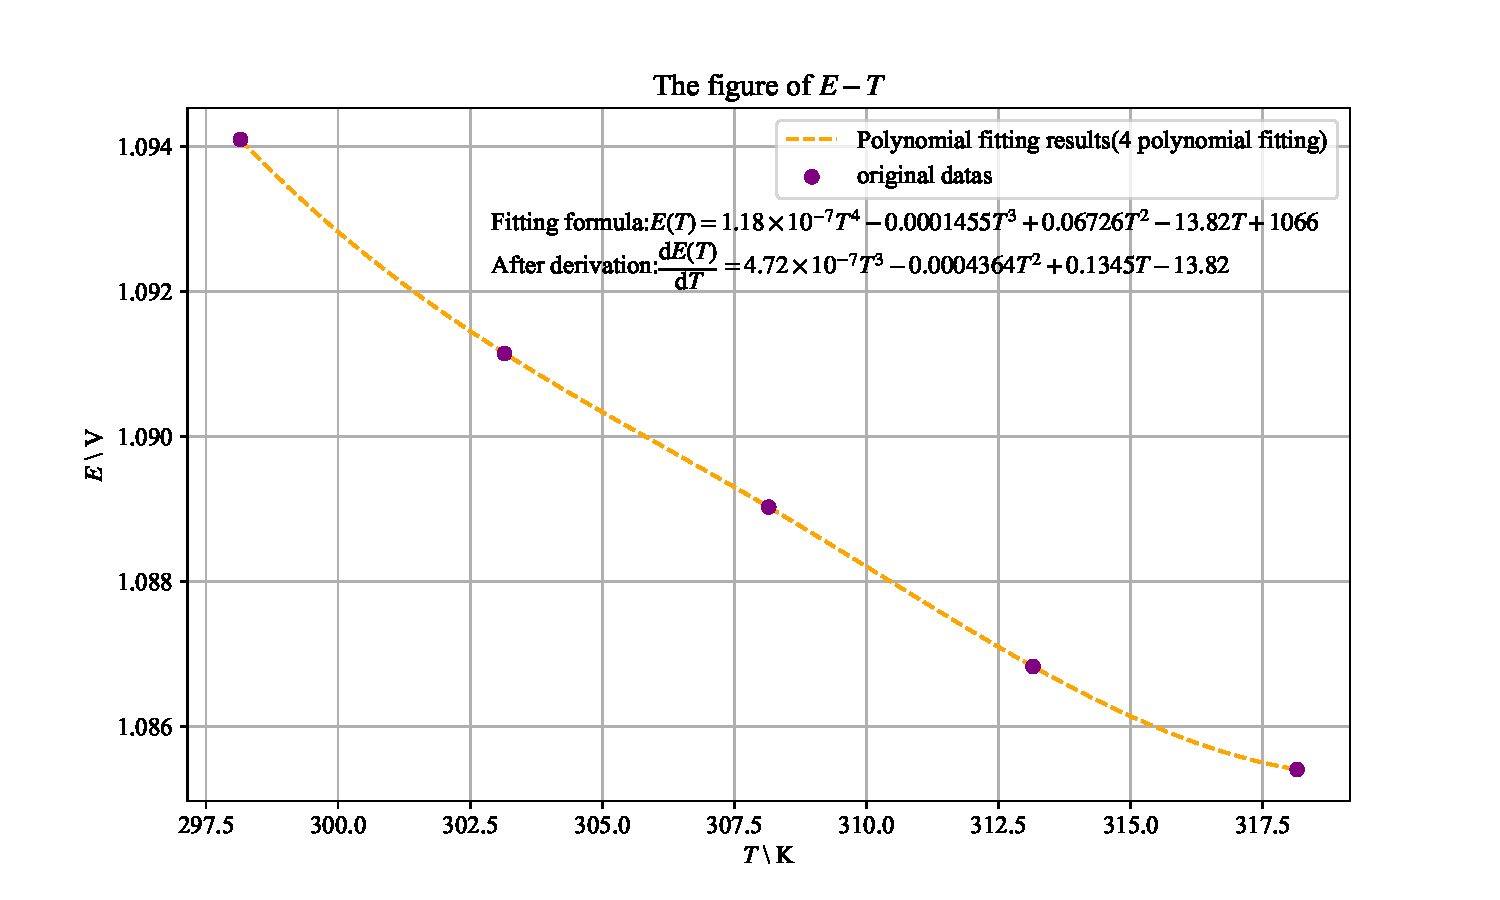
\includegraphics[scale=0.63]{6}
	\caption{利用四次多项式拟合得到的$E-T$曲线,其中横坐标为热力学温度$T$(单位:开尔文 K),纵坐标为原电池$\ce{Zn}_{(\rm{s}})|\ce{ZnSO4}(0.1\rm{mol}/L)||\ce{CuSO4}(0.1\rm{mol/L})|\ce{Cu}_{(\rm{s})}$的电池电动势 $E$(单位:伏特 V)。多项式拟合结果为:\textcolor[rgb]{0.54,0.13,0.33}{$E(T) =1.18\times 10^{-7} T^{4} - 0.0001455 T^{3} + 0.06726 T^{2} - 13.82 T + 1066$},公式中的 $E(T)$与$T$视作无量纲数,即:$E(T) = \dfrac{E(T)}{\ce{V}}$,$T = \dfrac{T}{\ce{K}}$,上式两边对温度$T$求一阶导数,$E(T)$恒压下为温度$T$的函数,得:\textcolor[rgb]{0.54,0.13,0.33}{$\pqty{\dfrac{\partial E}{\partial T}}_{p} = \dfrac{{\rm{d}}E(T)}{{\rm{d}}T} = 4.72\times 10^{-7} T^{3} - 0.0004364 T^{2} + 0.1345 T - 13.82$}。}
	\label{fi1}
\end{figure}
\newpage
\section{实验七:溶液表面张力的测定}
\begin{figure}[h]
	\centering
	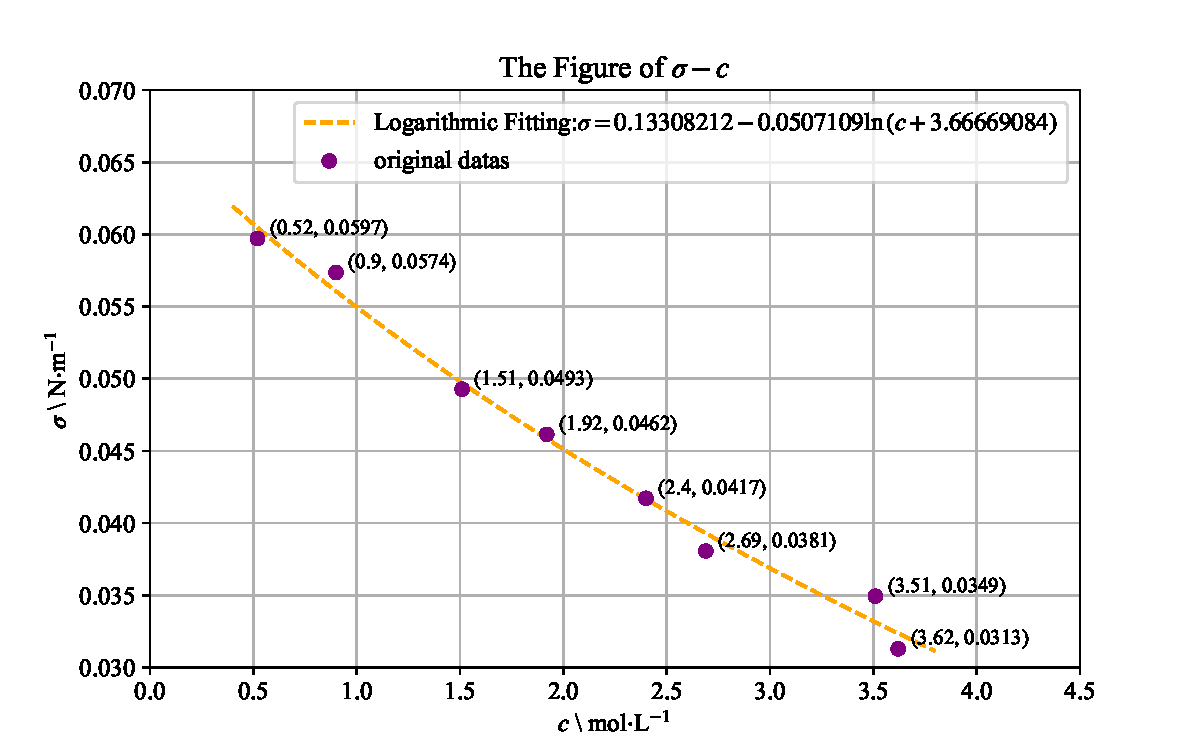
\includegraphics[scale=0.8]{Figure1}
	\caption{利用函数$\sigma = a + b \ln{(c + d)}$拟合得到的$\sigma - c$曲线。其中$a,b,d$均为参数,$c$为乙醇溶液的浓度(去除单位为:mol$\cdot$m$^{-1}$),$\sigma$为溶液表面张力(去除单位为:N$\cdot$m$^{-2}$)得到的拟合拟合结果为:\textcolor[rgb]{0.54,0.13,0.33}{$ \sigma= 0.13308212+0.0507109\ln{(c + 3.66669084)}$},回归系数$R^{2} = 0.993$。}
	\label{fi2}
\end{figure}
\newpage
\begin{figure}[h]
	\centering
	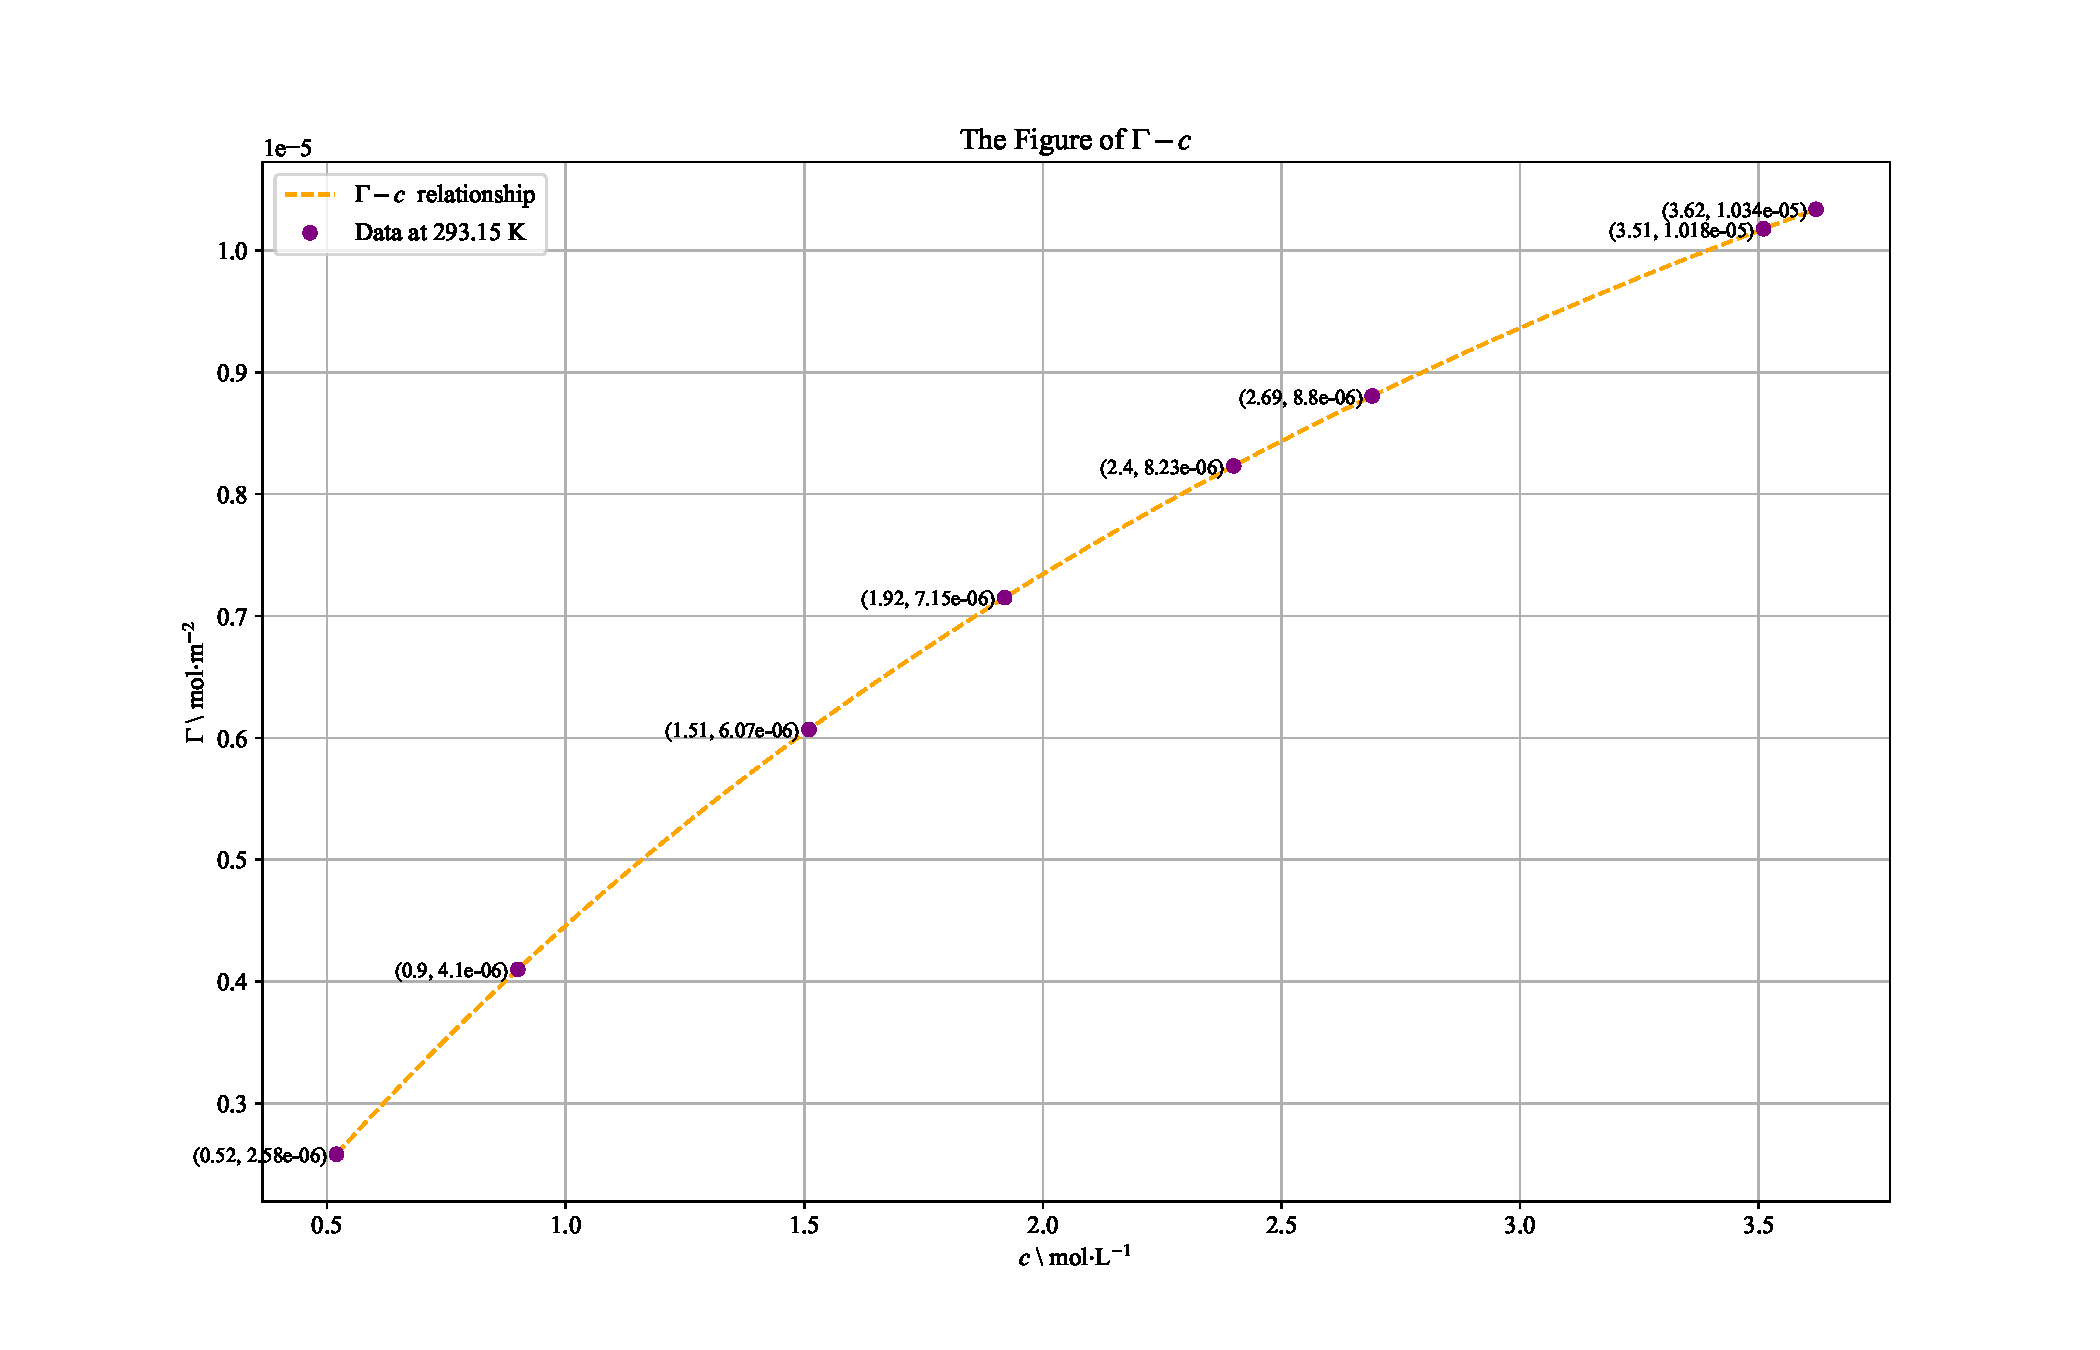
\includegraphics[scale=0.8]{Figure2}
	\caption{利用$\sigma - c$的拟合结果求出$\varGamma - c$曲线。其中$\varGamma$是溶质在表面层的吸附量(去除单位为 mol$\cdot$ m$^{-2}$,纵坐标为$1\times 10^{-5}$mol$\cdot$ m$^{-2}$),计算公式为\textcolor[rgb]{0.07,0.36,0.57}{$\varGamma = \dfrac{c}{RT}\pqty{\dfrac{\rm{d}\sigma}{\rm{d}c}}_{T}$},其中 $T$取实验温度$T = 293.15$K。}
	\label{fi3}
\end{figure}

\begin{figure}[h]
	\centering
	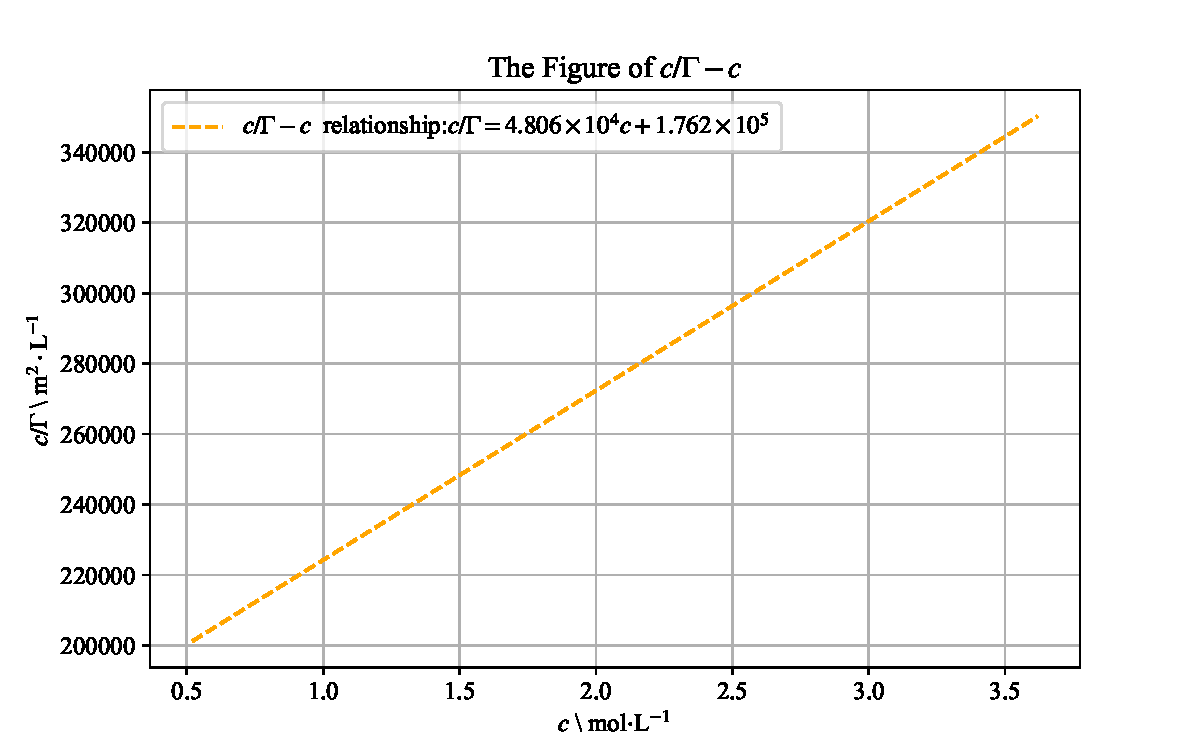
\includegraphics[scale=0.8]{Figure3}
	\caption{$\dfrac{c}{\varGamma}-c$关系图,纵坐标为$\dfrac{c}{\varGamma}$(去单位为m$^{-1}$),横坐标为$c$(去单位为 mol$\cdot $m$^{-3}$)。利用一次拟合,得到一直线,关系式为\textcolor[rgb]{0.54,0.13,0.33}{$\dfrac{c}{\varGamma} = 4.806 \times 10^{4}c + 1.762 \times 10^{8}$},应符合关系式\textcolor[rgb]{0.07,0.36,0.57}{$\dfrac{c}{\varGamma} = \dfrac{c}{\varGamma_{\infty}}+\dfrac{1}{K\varGamma_{\infty}}$},故其斜率之倒数为$\varGamma_{\infty} = 2.081 \times10^{-5}$mol$\cdot$ m$^{-2}$}
	\label{fi4}
\end{figure}
\newpage
\section{实验八:弱电解质电离平衡常数的测定}
\begin{figure}[h]
	\centering
	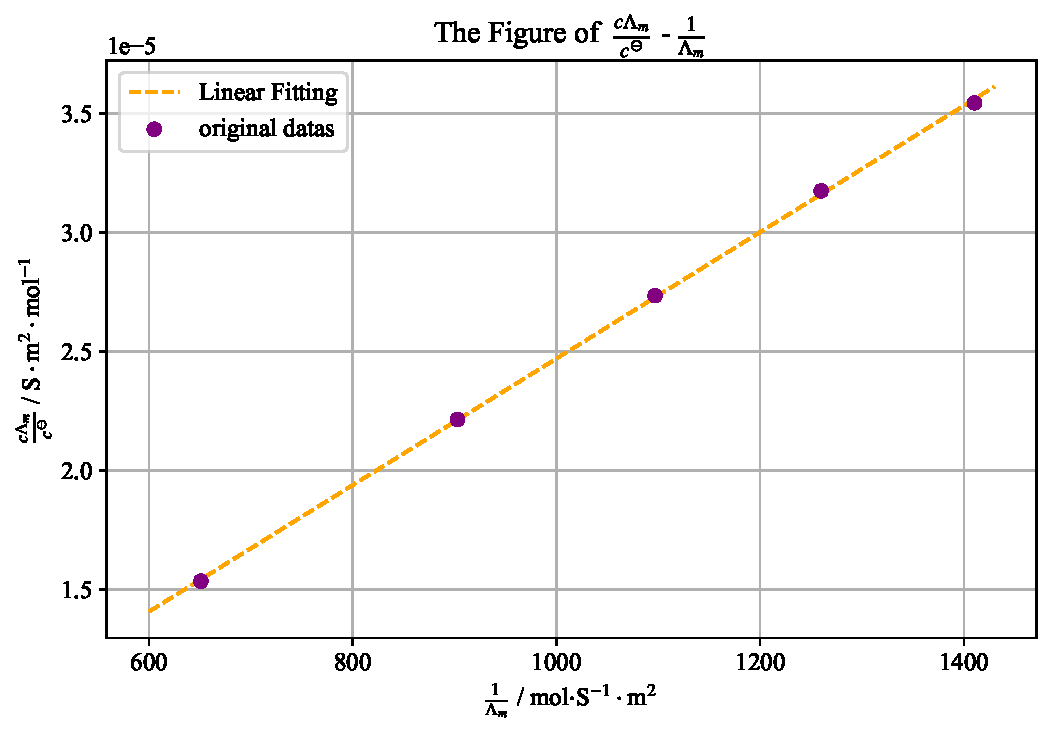
\includegraphics[scale=0.8]{Map}
	\caption{$\dfrac{c\varLambda_{m}}{c^{\ominus}} $(去单位为$\rm{S}\cdot\rm{m}^{2}\cdot\rm{mol}^{-1}$)对$ \dfrac{1}{\varLambda_{m}}$(去单位为$\rm{mol}\cdot\rm{S}^{-1}\cdot\rm{m}^{-2}$)作图,得到的方程为\textcolor[rgb]{0.54,0.13,0.33}{$\dfrac{c\varLambda_{m}}{c^{\ominus}} =2.657\times 10^{-8} \dfrac{1}{\varLambda_{m}}- 1.867\times 10^{-6}$},用斜率除以$\varLambda_{m,\infty}^{2}$,就得到\textcolor[rgb]{0.54,0.13,0.33}{$K_{c}^{\ominus} = 1.741\times 10^{-5}$}。}
	\label{fi5}
\end{figure}
\end{document}
